% Compile twice with pdfLaTeX from this directory to resolve the criterion links.
\makeatletter
\def\input@path{{../../../preamble/}{book2026-2027/preamble/}}
\makeatother
\input{preamble.tex}
\input{graphs/highlights.tex}
% \GTenHighlightsfalse % Uncomment to disable instructional highlights.
\input{graphs/specific_highlights.tex}

\geometry{letterpaper,margin=0.72in}
\linespread{1.06}
\setlength{\parskip}{4pt minus 3pt}
\setcounter{secnumdepth}{1}
\setlist[enumerate]{leftmargin=1.75em,topsep=3pt,itemsep=2pt,parsep=0pt}
\hypersetup{pdftitle={Grade 11 Global Economics --- Term 2 Review Outline},
  linkcolor=taskLinkDarkBlue}
\newcolumntype{Y}{>{\raggedright\arraybackslash}X}
\newcolumntype{P}[1]{>{\raggedright\arraybackslash}p{#1}}
\newcommand{\Cue}[1]{\textbf{Use when} #1\par}
\newcommand{\Example}[1]{\smallskip\textbf{#1}\enspace\ignorespaces}
% Compact strokes for the outline's tables and side-by-side examples.
\tikzset{gten marker/.append style={inner xsep=0.7mm,inner ysep=0.35mm}}
\newcommand{\SampleGroup}[1]{\HighlightStroke{G11T2C1Sample}{#1}}
\newcommand{\PopulationGroup}[1]{\HighlightStroke{G11T2C1Population}{#1}}
\newcommand{\SampleMean}[1]{\HighlightStroke{G11T2C1SampleMean}{#1}}
\newcommand{\PopulationMean}[1]{\HighlightStroke{G11T2C1PopulationMean}{#1}}
\newcommand{\SampleSD}[1]{\HighlightStroke{G11T2C1SampleSD}{#1}}
\newcommand{\PopulationSD}[1]{\HighlightStroke{G11T2C1PopulationSD}{#1}}
\newcommand{\SampleShare}[1]{\HighlightStroke{G11T2C1SampleProportion}{#1}}
\newcommand{\PopulationShare}[1]{\HighlightStroke{G11T2C1PopulationProportion}{#1}}
\newcommand{\Margin}[1]{\HighlightStroke{GTenHLValue}{#1}}
\newcommand{\Endpoint}[1]{\HighlightStroke{GTenHLProbability}{#1}}
\newcommand{\MethodCue}[1]{\HighlightStroke{GTenHLOutcome}{#1}}
\tikzset{
  review segment/.style={blue!65!black},
  review endpoint/.style={},
  review estimate/.style={},
  review margin/.style={},
  review label/.style={}
}
\pgfplotsset{
  review plot/.style={axis lines=left,scaled ticks=false,
    tick label style={font=\small},label style={font=\small}},
  review interval/.style={blue!65!black,thick,mark=|},
  review reference/.style={black,dashed},
  review fixed mean/.style={review reference},
  review sample share/.style={review reference},
  review sample mean/.style={blue!65!black,only marks,mark=*}
}
\ifGTenHighlights
  \tikzset{
    review segment/.append style={draw=GTenHLProbability!55!black},
    review endpoint/.append style={draw=GTenHLProbability!55!black},
    review estimate/.append style={fill=G11T2C1Sample},
    review margin/.append style={draw=GTenHLValue!55!black},
    review label/.append style={fill=#1!32!white,rounded corners=1mm}
  }
  \pgfplotsset{
    review interval/.append style={GTenHLProbability!55!black},
    review fixed mean/.append style={G11T2C1PopulationMean!65!black},
    review sample share/.append style={G11T2C1SampleProportion!65!black},
    review sample mean/.append style={G11T2C1SampleMean!55!black}
  }
\fi

\begin{document}
\begin{center}
  {\LARGE\bfseries Grade 11 Global Economics\\[2pt]--- Term 2 Review Outline\par}
  \smallskip
  {\large 2026--2027\par}
\end{center}

\setcounter{tocdepth}{1}
\phantomsection
\label{toc}
\tableofcontents

\section{Introduction}

In Lesson 1 (C1--C4), you describe samples and populations, then use a sample to estimate a population mean. In Lesson 2 (C5--C7), you estimate a population proportion, plan sample sizes and compare precision with confidence. In Lesson 3 (C8--C10), you estimate a mean when the population spread is unknown, audit an inference and decide what a study supports.

\textbf{A routine for any question}
\begin{enumerate}
  \item Define the target population, its time window and one observational unit. Name the population parameter in context.
  \item Identify the corresponding sample statistic and its units.
  \item Check how the sample was selected and whether the proposed procedure's assumptions are reasonable.
  \item Calculate the estimate and its precision. For an interval, show the standard error, cutoff, margin and both endpoints. Carry unrounded values until reporting.
  \item Explain the result for the population, with units. If there is a benchmark, say what the interval supports and what remains open.
\end{enumerate}

\par\nobreak
\secInicio

\clearpage
\section{Summarized Outline}\label{sec:summary}

Match the question to a row. Select a criterion to jump to its worked example.

{\small\noindent
\begin{tabularx}{\linewidth}{@{}l P{0.25\linewidth} P{0.25\linewidth} Y@{}}
  \toprule
  & \textbf{Question cue} & \textbf{Method} & \textbf{Show in your work}\\
  \midrule
  \TaskHyperref{crit:c1}{\textbf{C1}} & Who or what is described? & Match parameters to statistics & Population, unit, sample, symbols and changes\\
  \TaskHyperref{crit:c2}{\textbf{C2}} & What does 95\% confidence mean? & Compare point and interval estimates & Centre, half-width and count crossing the fixed mean\\
  \TaskHyperref{crit:c3}{\textbf{C3}} & What controls the width? & Decompose the interval & Label centre, margin and endpoints. Shade central area and mark tails.\\
  \TaskHyperref{crit:c4}{\textbf{C4}} & Estimate a mean with known variance & One-sample mean \(z\) interval & Convert variance to SD. Show checks, cutoff and endpoints.\\
  \TaskHyperref{crit:c5}{\textbf{C5}} & Estimate a share from a count & One-proportion \(z\) interval & Event, both counts, estimated SE, margin and percent endpoints\\
  \TaskHyperref{crit:c6}{\textbf{C6}} & How many usable records? & Solve \(E\le E_{\rm target}\) & Bound, round up, check feasibility and verify precision\\
  \TaskHyperref{crit:c7}{\textbf{C7}} & Confidence or sample size changes & Compare \(E=z^*\widehat{SE}\) & Compare widths and identify which factor explains the change\\
  \TaskHyperref{crit:c8}{\textbf{C8}} & Estimate a mean with unknown \(\sigma\) & One-sample Student's \(t\) interval & Shape check, \(df\), cutoff, \(s/\sqrt n\) and endpoints\\
  \TaskHyperref{crit:c9}{\textbf{C9}} & Can we trust this interval? & Audit design and assumptions & Name the concern, evidence and defensible next step\\
  \TaskHyperref{crit:c10}{\textbf{C10}} & Plan, analyse and report a study & Connect design, interval and decision & Target population, planned \(n\), achieved margin, benchmark and scope\\
  \bottomrule
\end{tabularx}\par
}

\clearpage
\enlargethispage{12pt}
\textbf{Notation at a glance}

The table pairs \SampleGroup{sample statistics (green)} with
\PopulationGroup{population parameters (red)}. Each row has its own shades.
\Margin{Amber} marks margins and widths, \Endpoint{blue} marks endpoints and
interval segments, and \MethodCue{lavender} marks cues for choosing or applying a method.

{\small\noindent
\begin{tabularx}{\linewidth}{@{}P{0.22\linewidth}YY@{}}
  \toprule
  \textbf{Quantity} & \PopulationGroup{\textbf{Population parameter}} & \SampleGroup{\textbf{Sample statistic}}\\
  \midrule
  Mean & \(\PopulationMean{\mu}\), population mean & \(\SampleMean{\bar x}\), sample mean\\
  Standard deviation (SD) & \(\PopulationSD{\sigma}\), population SD & \(\SampleSD{s}\), sample SD (variance uses \(n-1\))\\
  Proportion & \(\PopulationShare{p}\), population share with the event & \(\SampleShare{\hat p}=x/n\), observed share from \(x\) events\\
  \bottomrule
\end{tabularx}\par
}

\textbf{Choose the interval.} Check random selection from a frame that covers the population. For a simple random sample without replacement, \(n/N\le 0.10\) supports approximate independence (\(n\) is sample size, \(N\) is population size). Check separately for dependence within groups.

{\small
\setlength{\tabcolsep}{4pt}
\noindent
\begin{tabularx}{\linewidth}{@{}P{0.17\linewidth}cclY@{}}
  \toprule
  \textbf{Method} & \textbf{Target} & \textbf{Standard error} & \textbf{Critical value} & \textbf{Additional checks}\\
  \midrule
  Known-\(\PopulationSD{\sigma}\) mean \(z\) & \(\PopulationMean{\mu}\) & \(\PopulationSD{\sigma}/\sqrt n\) & \(z^*\) & Quantitative data, \MethodCue{known population SD} and an approximately normal model for \(\bar x\).\\
  One-proportion \(z\) & \(\PopulationShare{p}\) & \(\sqrt{\SampleShare{\hat p}(1-\hat p)/n}\) & \(z^*\) & \MethodCue{Binary outcome} with at least \MethodCue{10 events and 10 non-events} in the sample.\\
  Unknown-\(\PopulationSD{\sigma}\) mean \(t\) & \(\PopulationMean{\mu}\) & \(\SampleSD{s}/\sqrt n\) & \(t^*\), \(df=n-1\) & Quantitative data. For small samples, look for \MethodCue{rough symmetry} and \MethodCue{no influential outliers}.\\
  \bottomrule
\end{tabularx}\par
}

\begin{center}
\begin{tikzpicture}[x=1cm,y=0.70cm,font=\small,>=Stealth]
  \draw[thick,review segment] (0,0)--(8,0);
  \draw[thick,review endpoint] (0,-.13)--(0,.13) (8,-.13)--(8,.13);
  \fill[review estimate] (4,0) circle (2pt);
  \node[below=3pt,review label=GTenHLProbability] at (0,0) {Lower endpoint \(\text{estimate}-E\)};
  \node[below=3pt,review label=G11T2C1Sample] at (4,0) {Point estimate};
  \node[below=3pt,review label=GTenHLProbability] at (8,0) {Upper endpoint \(\text{estimate}+E\)};
  \draw[<->,review margin] (0,.40)--node[above,review label=GTenHLValue]{Margin \(E\)}(4,.40);
  \draw[<->,review margin] (4,.40)--node[above,review label=GTenHLValue]{Margin \(E\)}(8,.40);
  \draw[<->,review margin] (0,1.19)--node[above,review label=GTenHLValue]{Full width \(2E\)}(8,1.19);
\end{tikzpicture}
\end{center}
\par\nobreak
\secInicio

\section{Step-by-Step Outline}

\subsection{C1 --- Identify parameters and sample statistics}\label{crit:c1}
\Cue{the question asks whose data you have and whose characteristics you want to describe.}
\begin{enumerate}
  \item Name the unit, the full group eligible in the stated period and the units actually observed.
  \item Name the quantitative measure and the event. Pair \(\PopulationMean{\mu}\) with \(\SampleMean{\bar x}\), \(\PopulationSD{\sigma}\) with \(\SampleSD{s}\) and \(\PopulationShare{p}\) with \(\SampleShare{\hat p}\).
  \item Decide whether the draw or the population definition changed. Subtract sample statistics in their own units and report share differences in percentage points (pp).
\end{enumerate}

\Example{Market stalls.} One stall is one unit. The population is \PopulationGroup{all 1,200 stalls} licensed for June. Here \(\PopulationMean{\mu}\) and \(\PopulationSD{\sigma}\) describe the mean and SD of June sales, and \(\PopulationShare{p}\) is the share accepting digital payment. In the first \SampleGroup{random sample of 60}, \(\SampleMean{\bar x}=\SampleMean{4.8}\) and \(\SampleSD{s}=\SampleSD{1.2}\) million COP, with \(\SampleShare{\hat p}=18/60=\SampleShare{30\%}\). A fresh draw gives \SampleMean{5.1}, \SampleSD{1.0} and \SampleShare{25\%}. The differences (second minus first) are \(5.1-4.8=\SampleMean{+0.3}\) and \(1.0-1.2=\SampleSD{-0.2}\) million COP, and \(25\%-30\%=\SampleShare{-5}\) pp. The samples differ while the June population parameters are fixed.

\Example{Transit routes.} The unit is one Monday boarding. Adding suburban routes expands the population from \PopulationGroup{8,400 to 12,000} boardings, so fare \(\PopulationMean{\mu},\PopulationSD{\sigma}\) and discounted-fare \(\PopulationShare{p}\) now refer to the combined routes. Separate \SampleGroup{draws of 100} give changes of \(3.4-3.2=\SampleMean{0.2}\) in \(\SampleMean{\bar x}\) and \(0.9-0.8=\SampleSD{0.1}\) in \(\SampleSD{s}\) (thousand COP). The discounted share changes by \(0.30-0.35=\SampleShare{-0.05}\), or \(-5\) pp. The population differences are unknown.
\par\nobreak
\secInicio[][sec:summary]

\clearpage
\subsection{C2 --- Interpret point estimates and confidence}\label{crit:c2}
\Cue{a report gives a single estimate, a confidence interval or a claim about coverage.}
\begin{enumerate}
  \item Identify the point estimate and the population quantity it estimates. Read the interval as a range for that same quantity and find its half-width.
  \item On a repeated-sampling plot, count the intervals that cross the fixed parameter line and divide by the number of intervals shown.
  \item Explain the stated confidence level as long-run coverage under the same sampling and model conditions.
\end{enumerate}

\noindent
\begin{minipage}[t]{0.46\linewidth}
\vspace{0pt}
\Example{Weekly market fees.} The city's random sample gives \(\SampleMean{\bar x}=\SampleMean{106}\) for the mean weekly stall fee. The 95\% interval \([\Endpoint{101},\Endpoint{111}]\) has margin \((111-101)/2=\Margin{5}\). All amounts are in thousand COP.

In the simulation, samples 1, 2, 3 and 5 cover \(\PopulationMean{\mu}=\PopulationMean{104}\). Sample 4 misses because its lower endpoint is 105. The observed coverage is \(4/5=80\%\).
\end{minipage}\hfill
\begin{minipage}[t]{0.51\linewidth}
\vspace{0pt}
\centering
% Repeated draws and fixed mean from the C2 practice.
\begin{tikzpicture}
  \begin{axis}[review plot,width=\linewidth,height=4.6cm,
    xmin=98,xmax=116,ymin=0.6,ymax=5.6,
    xlabel={Mean weekly fee (thousand COP)},ylabel={Sample},
    ytick={1,2,3,4,5},xtick={99,104,109,114}]
    \addplot[review fixed mean] coordinates {(104,0.6) (104,5.6)};
    \addplot[review interval] coordinates {(101,1) (111,1)};
    \addplot[review interval] coordinates {(99,2) (109,2)};
    \addplot[review interval] coordinates {(103,3) (113,3)};
    \addplot[review interval] coordinates {(105,4) (115,4)};
    \addplot[review interval] coordinates {(102,5) (112,5)};
    \node[font=\small,review label=G11T2C1PopulationMean] at (axis cs:100.8,4.0) {$\mu=104$};
  \end{axis}
\end{tikzpicture}
\end{minipage}

Over many fresh samples, about 95\% of intervals made by this procedure should contain the fixed mean. Five draws can give a different fraction. Once \([101,111]\) is calculated, the endpoints and mean are fixed. This particular interval either covers the mean or misses it, so assigning it a 95\% probability of coverage misreads the confidence level.
\par\nobreak
\secInicio[][sec:summary]

\subsection{C3 --- Explain the parts of an interval}\label{crit:c3}
\Cue{you need to label an interval, find a cutoff or explain a change in precision.}
\begin{enumerate}
  \item Use the point estimate as the centre. The standard error measures the typical sampling variation of the statistic.
  \item For central confidence \(C\) as a decimal, sketch equal tails of area \((1-C)/2\). Find the positive cutoff using central area \(C\) or left cumulative area \((1+C)/2\).
  \item Multiply the cutoff by the standard error for \(\Margin{E}\). Write both endpoints as estimate \(\pm E\) and the full width as \(2E\).
\end{enumerate}

\noindent
\begin{minipage}[t]{0.50\linewidth}
\vspace{0pt}
\centering
% The C3 practice curve, with both tail areas labeled.
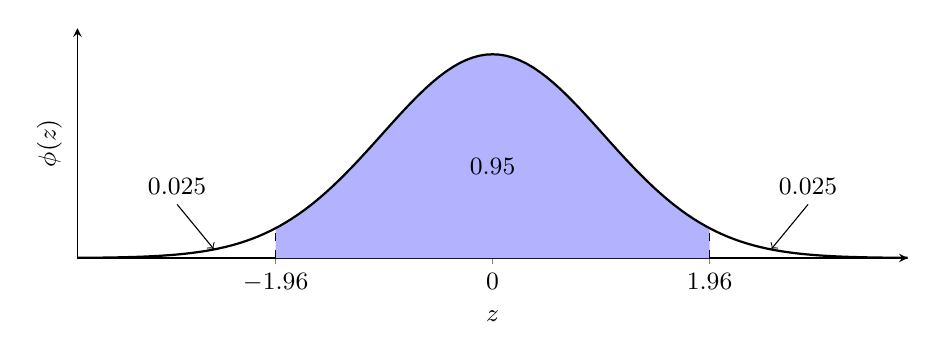
\begin{tikzpicture}
  \begin{axis}[review plot,width=\linewidth,height=4.5cm,
    xmin=-3.75,xmax=3.75,ymin=0,ymax=0.45,
    xlabel={$z$},ylabel={$\phi(z)$},xtick={-1.96,0,1.96},
    xticklabels={$-1.96$,$0$,$1.96$},ytick=\empty]
    \addplot[draw=none,fill=blue!30,domain=-1.96:1.96,samples=85]
      {exp(-x^2/2)/sqrt(2*pi)} \closedcycle;
    \addplot[black,thick,domain=-3.75:3.75,samples=125] {exp(-x^2/2)/sqrt(2*pi)};
    \addplot[review reference] coordinates {(-1.96,0) (-1.96,0.05844)};
    \addplot[review reference] coordinates {(1.96,0) (1.96,0.05844)};
    \node[font=\small] at (axis cs:0,0.18) {$0.95$};
    \node[font=\small] at (axis cs:-2.85,0.14) {$0.025$};
    \node[font=\small] at (axis cs:2.85,0.14) {$0.025$};
    \draw[->] (axis cs:-2.85,0.105)--(axis cs:-2.52,0.018);
    \draw[->] (axis cs:2.85,0.105)--(axis cs:2.52,0.018);
  \end{axis}
\end{tikzpicture}
\end{minipage}\hfill
\begin{minipage}[t]{0.47\linewidth}
\vspace{0pt}
\Example{Weekly groceries.} The district's sample gives centre \SampleMean{84} and \(SE=3\), both in thousand COP. Central area 0.95 gives left area \(0.975\) at \(z^*=1.96\).
\[
  E=1.96(3)=\Margin{5.88},\qquad 2E=11.76.
\]
The 95\% interval for the mean weekly grocery bill is \(\SampleMean{84}\pm\Margin{5.88}=[\Endpoint{78.12},\Endpoint{89.88}]\) thousand COP.
\end{minipage}

With the same data, 90\% confidence gives \(E=1.645(3)=4.935\) and width \(9.87\) thousand COP. The centre stays at 84 and nominal coverage falls. With confidence fixed, halving \(SE\) halves the margin and width. With \(SE\) and confidence fixed, a centre 4 thousand COP higher moves both endpoints up by 4 and preserves the width.
\par\nobreak
\secInicio[][sec:summary]

\clearpage
\enlargethispage{12pt}
\subsection{C4 --- Estimate a mean with known variance}\label{crit:c4}
\Cue{the response is \MethodCue{quantitative} and the population \MethodCue{variance or SD is given}.}
\begin{enumerate}
  \item Define \(\PopulationMean{\mu}\) and record \(\SampleMean{\bar x},n\) and the known variance \(\PopulationSD{\sigma^2}\). Take \(\PopulationSD{\sigma}=\sqrt{\sigma^2}\) to return to the units of the data.
  \item Check random selection and the sampling fraction for sampling without replacement. A bell-shaped population supports normality of \(\SampleMean{\bar x}\). For other shapes, check that the sample is large enough for a normal approximation given the skew and any extreme values.
  \item Compute \(SE(\SampleMean{\bar x})=\PopulationSD{\sigma}/\sqrt n\). For a two-sided interval, read \(z^*\) from the central area or the cumulative area to its left.
  \item Calculate \(E=z^*SE\), then \(\SampleMean{\bar x}-E\) and \(\SampleMean{\bar x}+E\). Report the range for the mean in context and locate any benchmark.
\end{enumerate}

\Example{Warehouse handling charges.} Let \(\PopulationMean{\mu}\) be the mean charge per pallet across the 1,200 pallets in the quarter. One receipt represents one pallet. The \SampleGroup{36 receipts} form a simple random sample without replacement, with \(36/1{,}200=3\%\). The population is assumed approximately bell-shaped. With \(\SampleMean{\bar x}=\SampleMean{74}\) USD per pallet and \(\PopulationSD{\sigma^2}=\PopulationSD{144}\) in squared dollars,
\[
  \PopulationSD{\sigma}=\sqrt{144}=\PopulationSD{12},\qquad SE=\frac{\PopulationSD{12}}{\sqrt{36}}=2\text{ USD per pallet}.
\]
For central 99\%, each tail is \(0.01/2=0.005\). Read \(P(Z\le z^*)=0.995\), which gives \(z^*=2.576\).
\[
  E=2.576(2)=\Margin{5.152},\qquad
  [\SampleMean{74}-\Margin{5.152},\ \SampleMean{74}+\Margin{5.152}]=[\Endpoint{68.848},\Endpoint{79.152}].
\]
We are 99\% confident that the mean quarterly handling charge was about 68.85 to 79.15 USD per pallet. The upper endpoint is below 80 USD, giving evidence that the quarter's mean was below the proposed budget benchmark.
\par\nobreak
\secInicio[][sec:summary]

\subsection{C5 --- Estimate a population proportion}\label{crit:c5}
\Cue{each observation is classified by whether a \MethodCue{specified event} happened.}
\begin{enumerate}
  \item Define the event and its population proportion \(\PopulationShare{p}\). From \(x\) events in \(n\) records, compute \(\SampleShare{\hat p}=x/n\).
  \item Check random selection and the sampling fraction for sampling without replacement. Check that the \emph{observed} counts \(n\SampleShare{\hat p}\) and \(n(1-\SampleShare{\hat p})\) are both \MethodCue{at least 10}.
  \item Calculate \(\widehat{SE}=\sqrt{\SampleShare{\hat p}(1-\SampleShare{\hat p})/n}\), find \(z^*\) for the central confidence level and compute \(E=z^*\widehat{SE}\).
  \item Use \(\SampleShare{\hat p}-E\) and \(\SampleShare{\hat p}+E\). Multiply each endpoint by 100 to report a percent and multiply \(E\) by 100 to report a margin in percentage points.
\end{enumerate}

\Example{First-year microloan defaults.} Let \(\PopulationShare{p}\) be the share of the \PopulationGroup{8,000 small-business loans} in the cohort that defaulted within their first year. The \SampleGroup{400 loans} were randomly sampled without replacement and all have complete follow-up. The fraction is \(400/8{,}000=5\%\). The 50 defaults and \(400-50=350\) non-defaults both meet the count requirement.
\[
\begin{aligned}
  \SampleShare{\hat p}&=50/400=\SampleShare{0.125}, &
  \widehat{SE}&=\sqrt{\SampleShare{0.125}(0.875)/400}\approx0.01654,\\
  E&=2.326\sqrt{0.125(0.875)/400}\approx\Margin{0.03846}, &
  \SampleShare{\hat p}\pm \Margin{E}&\ \Longrightarrow\ [\Endpoint{0.08654},\Endpoint{0.16346}]\ \text{(approx.)}.
\end{aligned}
\]
The 98\% cutoff \(2.326\) comes from left area 0.990. The estimate is 12.5\%, with a margin of 3.85 pp. We are 98\% confident that about 8.65\% to 16.35\% of the cohort defaulted within a year. The interval lies below the 20\% benchmark.
\par\nobreak
\secInicio[][sec:summary]

\clearpage
\subsection{C6 --- Plan sample size for a target margin}\label{crit:c6}
\Cue{the study specifies confidence and a \MethodCue{maximum margin} before collecting data.}
\begin{enumerate}
  \item Set \(E_{\rm target}\) in the response units for a mean or as a decimal proportion for a share. Choose the cutoff for the planned confidence level.
  \item Write the margin as \(z^*A/\sqrt n\). Use \(A=\PopulationSD{\sigma}\) for a known-SD mean or \(A=\sqrt{p_0(1-p_0)}\) for a share, where \(p_0\) is the \MethodCue{planning value}. Then
  \[
    \frac{z^*A}{\sqrt n}\le E_{\rm target}
    \quad\Longrightarrow\quad \sqrt n\ge\frac{z^*A}{E_{\rm target}}
    \quad\Longrightarrow\quad n\ge\left(\frac{z^*A}{E_{\rm target}}\right)^2.
  \]
  \item Round up to the minimum whole number of usable records. Plan random selection and check the sampling fraction. For a share, check that \(np_0\) and \(n(1-p_0)\) are each at least 10. For a mean, assess whether the planned sample and anticipated shape support the method.
  \item After collection, check the usable \(n\), the design and sampling fraction, and the observed counts or shape. Recompute the margin with the analysis method and compare with the target.
\end{enumerate}

\Example{Port inspections.} The target for mean clearance time is 3 min at 95\% confidence. With known \(\PopulationSD{\sigma}=\PopulationSD{12}\) min, the bound is \((1.96\cdot12/3)^2=61.4656\). The large list supports independent records and a normal approximation is suitable.
\[
  E(62)=\frac{23.52}{\sqrt{62}}\approx\Margin{2.987}\text{ min},\qquad
  E(61)=\frac{23.52}{\sqrt{61}}\approx\Margin{3.011}\text{ min}.
\]
The margin decreases with \(n\), so 62 is the smallest sample that meets the cap.

\Example{Household subsidy share.} For a 95\% interval and a 4 pp cap, set \(E_{\rm target}=\Margin{0.04}\). A pilot suggests \(p_0=0.20\), giving \(1.96^2(0.20)(0.80)/0.04^2=384.16\), so plan for 385 households. The expected counts are 77 and 308 and \(385/20{,}000=1.925\%\). Without a dependable pilot, \(p_0=0.50\) maximizes \(p_0(1-p_0)\) at 0.25. The bound rises to 600.25, so plan for 601 households (about 3.0\% of the registry), with expected counts of 300.5 each at that planning share. This caps the formula's margin for any observed share. Check the actual counts before using the formula. For a pilot SD used to plan a mean study, see \TaskHyperref{crit:c10}{C10}.
\par\nobreak
\secInicio[][sec:summary]

\subsection{C7 --- Compare confidence and precision}\label{crit:c7}
\Cue{sample size, confidence level or both change.}
\begin{enumerate}
  \item Write the centre and compute the standard error for each case.
  \item Use the cutoff for each confidence level. Compute \(E=z^*\widehat{SE}\), endpoints \(\SampleShare{\hat p}\pm E\) and width \(2E\).
  \item Identify what changed in the product \(z^*\widehat{SE}\) and compare the result with the study's requirements.
\end{enumerate}

\clearpage
\enlargethispage{12pt}
\Example{C7 worked example --- Mobile ticketing.} Random \SampleGroup{samples of 100 and 400} from \PopulationGroup{20,000 eligible riders} each give \(\SampleShare{\hat p}=\SampleShare{0.40}\) for mobile-ticket use last week. The fractions are 0.5\% and 2\%, with counts of \(40,60\) and \(160,240\). Use \(\widehat{SE}=\sqrt{0.40(0.60)/n}\). In row C, \(E=2.576\sqrt{0.24/400}\approx\Margin{0.06310}\), so the interval is about \([\Endpoint{33.69\%},\Endpoint{46.31\%}]\).

\noindent
\begin{minipage}[t]{0.49\linewidth}
\vspace{0pt}
\centering
% The C7 practice comparison with its 400-rider, 99% variant added.
\begin{tikzpicture}
  \begin{axis}[review plot,width=\linewidth,height=4.7cm,
    xmin=29,xmax=51,ymin=0.55,ymax=3.55,ytick={1,2,3},
    yticklabels={A,B,C},xtick={30,35,40,45,50},
    xlabel={Mobile-ticket use (\%)}]
    \addplot[review sample share] coordinates {(40,0.55) (40,3.55)};
    \addplot[review interval] coordinates {(31.94118,1) (48.05882,1)};
    \addplot[review interval] coordinates {(35.97059,2) (44.02941,2)};
    \addplot[review interval] coordinates {(33.69011,3) (46.30989,3)};
    \node[anchor=south,font=\small,fill=white,inner sep=1pt,review label=G11T2C1SampleProportion]
      at (axis cs:40,3.11) {$\hat p=40\%$};
  \end{axis}
\end{tikzpicture}
\end{minipage}\hfill
\begin{minipage}[t]{0.49\linewidth}
\vspace{0pt}
\centering\small
\setlength{\tabcolsep}{3pt}
\begin{tabular}{@{}lrrrrrr@{}}
  \toprule
  & \(n\) & Conf. & \(z^*\) & \(\widehat{SE}\) & \(\Margin{E}\) (pp) & \(2\Margin{E}\) (pp)\\
  \midrule
  A & 100 & 90\% & 1.645 & 0.04899 & \Margin{8.06} & 16.12\\
  B & 400 & 90\% & 1.645 & 0.02449 & \Margin{4.03} & 8.06\\
  C & 400 & 99\% & 2.576 & 0.02449 & \Margin{6.31} & 12.62\\
  \bottomrule
\end{tabular}\par\smallskip
\raggedright
The dashed line marks the common centre. The segments run from \(\SampleShare{\hat p}-E\) to \(\SampleShare{\hat p}+E\) on the percent scale. A spans 31.94\% to 48.06\%, and B spans 35.97\% to 44.03\%.
\end{minipage}

\begin{itemize}[topsep=3pt,itemsep=2pt]
  \item \textbf{A to B, sample size only.} With the share and cutoff fixed, quadrupling \(n\) halves the SE and the width. B is more precise at the same 90\% confidence.
  \item \textbf{B to C, confidence only.} The same SE is multiplied by \(2.576\) instead of \(1.645\). C is wider and targets 99\% long-run coverage.
  \item \textbf{A to C, both change.} The halved SE more than offsets the larger cutoff since \(2.576/(2\cdot1.645)\approx0.78\). C is narrower and has higher nominal coverage. It is the only row with at least 95\% confidence and a margin below 7 pp.
\end{itemize}
\par\nobreak
\secInicio[][sec:summary]

\subsection{C8 --- Estimate a mean with unknown population SD}\label{crit:c8}
\Cue{the response is quantitative and the sample SD \(\SampleSD{s}\) estimates the \MethodCue{unknown} \(\PopulationSD{\sigma}\).}
\begin{enumerate}
  \item Define \(\PopulationMean{\mu}\), record \(\SampleMean{\bar x},\SampleSD{s},n\) and justify a one-sample Student's \(t\) interval. The proportion procedure is in \TaskHyperref{crit:c5}{C5}.
  \item Check random selection and \(n/N\) if sampling without replacement. Especially for small \(n\), inspect the shape for skew and influential outliers.
  \item Compute \(\widehat{SE}=\SampleSD{s}/\sqrt n\) and \(df=n-1\). Find \(t^*\) at that row and the required central area. In an upper-tail table, use the one-tail area \((1-C)/2\).
  \item Find \(E=t^*\widehat{SE}\) and report \([\SampleMean{\bar x}-E,\SampleMean{\bar x}+E]\) with confidence, units and population.
\end{enumerate}

\Example{Loading times.} The target is \(\PopulationMean{\mu}\), mean loading time for \PopulationGroup{all 400 eligible loads} in the month. A simple random \SampleGroup{sample of 12} distinct loads covers \(12/400=3\%\). Its dotplot is \MethodCue{roughly symmetric} with \MethodCue{no unusual values}, supporting a small-sample \(t\) interval. The mean is \SampleMean{84.60} min and the sample SD is \SampleSD{6.80} min.

\noindent
\begin{minipage}[t]{0.27\linewidth}
\vspace{0pt}
\centering\small
Central area\par\smallskip
\begin{tabular}{@{}rcc@{}}
  \toprule
  \(df\) & 90\% & 95\%\\
  \midrule
  11 & 1.796 & \MethodCue{\textbf{2.201}}\\
  12 & 1.782 & 2.179\\
  \bottomrule
\end{tabular}
\end{minipage}\hfill
\begin{minipage}[t]{0.69\linewidth}
\vspace{0pt}
At \(df=12-1=11\), central 95\% leaves 0.025 in each tail and gives \(t^*=\MethodCue{2.201}\).
\[
  \widehat{SE}=\frac{\SampleSD{6.80}}{\sqrt{12}}\approx1.9630\text{ min},\qquad
  E=2.201\left(\frac{\SampleSD{6.80}}{\sqrt{12}}\right)\approx\Margin{4.3205}\text{ min}.
\]
\end{minipage}

Using the unrounded margin, \(\SampleMean{84.60}\pm \Margin{E}\) gives about \([\Endpoint{80.28},\Endpoint{88.92}]\) minutes. We are 95\% confident that this range contains the mean loading time for the month's eligible loads. That is the average relevant to labour budgeting. Individual loading times can fall outside the interval.
\par\nobreak
\secInicio[][sec:summary]

\clearpage
\subsection{C9 --- Audit an inference before reporting it}\label{crit:c9}
\Cue{a proposed interval comes with a questionable design, rare outcomes, skew or unusual observations.}
\begin{enumerate}
  \item State the target population. Ask who could be selected, who actually responded and what might make their data different.
  \item Check independence. For a simple random sample without replacement, compute \(n/N\) and compare with 10\%. Check separately for grouping and repeated observations.
  \item Check both observed counts for a proportion. For a mean, check skew, sample size and the influence of unusual values.
  \item Match your next step to the problem. If the proposed interval is unsuitable, report a descriptive estimate and usable count for the observed group. Explain what limits population inference.
\end{enumerate}

{\small\noindent
\begin{tabularx}{\linewidth}{@{}P{0.19\linewidth}YY@{}}
  \toprule
  \textbf{Example} & \textbf{Concern and check} & \textbf{Defensible next step}\\
  \midrule
  \textbf{Card spending}\newline
  \SampleGroup{120 volunteers} from a target of \PopulationGroup{600 new customers}
  & Showing the survey only to budgeting-feature users creates \MethodCue{undercoverage}. Among users, \MethodCue{voluntary response} can select customers with different spending. Even a hypothetical simple random sample of 120 gives \(120/600=20\%\), above the guideline. Strong right skew and an unverified high value also warrant a shape check.
  & Describe the respondents and the recruitment method. For population inference, sample randomly from the full roster, use consistent records or follow up on missing responses, and verify the high value. Up to \(0.10(600)=60\) meets the fraction guideline for a simple random sample. For a larger draw, account for sampling without replacement.\\[3pt]
  \textbf{Rare defaults}\newline
  80 loans randomly drawn from 2,000
  & \(80/2{,}000=4\%\) passes the fraction check. There are 3 defaults and \(80-3=77\) non-defaults. Three is \MethodCue{below 10}, so the usual one-proportion \(z\) interval is unsuitable even with \(n>30\).
  & Report \(3/80=\SampleShare{3.75\%}\) among the audited loans. Use an interval suited to rare counts and the design. At this rate, expecting 10 defaults would take about \(10/0.0375\approx267\) loans, above \(0.10(2{,}000)=200\). A larger audit would need to account for that fraction and recheck actual counts.\\[3pt]
  \textbf{Freight invoices}\newline
  12 randomly drawn from 400
  & \(12/400=3\%\) passes the fraction check. A 510 USD charge among values near 100 USD can strongly affect \(\SampleMean{\bar x}\) and \(\SampleSD{s}\) in a sample of 12, undermining the small-sample \(t\) approximation.
  & Verify the invoice and eligibility. Keep a genuine eligible charge and assess its influence. Describe the sampled charges and the extreme observation. Consider a larger random sample or a method suited to skew.\\[3pt]
  \textbf{Freight variant}\newline
  Four sampled firms, three invoices per firm
  & \MethodCue{Shared contract rates} can make invoices from one firm similar. The overall 3\% fraction cannot establish approximate independence for this grouped design.
  & Account for grouping and selection probabilities in the analysis or draw a simple random sample from the full invoice list.\\
  \bottomrule
\end{tabularx}\par
}

\textbf{What the audit supports.} The bank can report the \SampleMean{mean spending} of its 120 respondents. More volunteers may make that description more stable while leaving both selection problems in place. A small margin calculated from a flawed design can still give a misleading picture of the population.
\par\nobreak
\secInicio[][sec:summary]

\clearpage
\subsection{C10 --- Design, analyse and report a study}\label{crit:c10}
\Cue{the question asks you to plan a study and decide what its evidence supports.}

\Example{Merchant fee revenue.} A bank wants to know whether the mean weekly net fee revenue per merchant under its payments package exceeds 12.90 thousand USD. It wants a two-sided 95\% interval with a margin at most 0.50 thousand USD per merchant.

\begin{enumerate}
  \item \textbf{Define the question and measurement.} The unit is one merchant. The population is the \PopulationGroup{500 small-business merchants} enrolled throughout the specified reference week. The parameter \(\PopulationMean{\mu}\) is the mean of their weekly net fee totals. Select distinct merchant IDs at random without replacement from the complete roster. Use one ledger total per merchant for that week, applying the same rebate and reversal rules. Include eligible zero-fee merchants and verify unusual totals.
  \item \textbf{Plan from the pilot.} Use the pilot SD of \SampleSD{0.90} thousand USD with \(z^*=1.96\) for an initial calculation.
  \[
    \frac{1.96(\SampleSD{0.90})}{\sqrt n}\le\Margin{0.50}
    \quad\Longrightarrow\quad
    n\ge\left(\frac{1.96(0.90)}{0.50}\right)^2=12.446784.
  \]
  The initial minimum is 13 usable records, \(13/500=2.6\%\) of the roster. The pilot SD is an estimate and the small-sample \(t\) cutoff will be larger than 1.96. Allow for extra records before collection and check the achieved margin afterwards.
  \item \textbf{Check the sample and calculate.} The bank randomly selected \SampleGroup{16 distinct merchants} before looking at revenues and obtained all 16 records. The fraction is \(16/500=3.2\%\). Values of 12, 13 and 14 thousand USD occur 4, 7 and 5 times. The \MethodCue{roughly symmetric} shape and lack of isolated extremes support a \(t\) interval, with limited information about shape from 16 observations. The quantitative response has \MethodCue{unknown} \(\PopulationSD{\sigma}\).
  \[
  \begin{aligned}
    \sum x_i &=4(12)+7(13)+5(14)=209,\qquad
    \sum x_i^2=4(12^2)+7(13^2)+5(14^2)=2739,\\
    \SampleMean{\bar x} &=209/16=\SampleMean{13.0625},\qquad
    \SampleSD{s}=\sqrt{\frac{2739-209^2/16}{15}}\approx\SampleSD{0.77190}.
  \end{aligned}
  \]
  At \(df=15\), the central 95\% cutoff is \(t^*=2.13145\).
  \[
    \widehat{SE}=\frac{\SampleSD{s}}{\sqrt{16}}\approx0.19298,\qquad
    E=2.13145\frac{\SampleSD{s}}{\sqrt{16}}\approx\Margin{0.41132},\qquad
    \SampleMean{\bar x}\pm \Margin{E}\ \Longrightarrow\ [\Endpoint{12.65},\Endpoint{13.47}].
  \]
  \item \textbf{Report precision and the benchmark decision.}

  \noindent
  \begin{minipage}[t]{0.50\linewidth}
  \vspace{0pt}
  \centering
  % The C10 practice benchmark plot, using the unrounded calculation.
  \begin{tikzpicture}
    \begin{axis}[review plot,width=\linewidth,height=4.15cm,
      xmin=12.45,xmax=13.65,ymin=0,ymax=1.8,
      xlabel={Mean weekly net fees (thousand USD)},
      xtick={12.5,12.9,13.5},xticklabels={12.50,12.90,13.50},ytick=\empty]
      \addplot[review reference] coordinates {(12.9,0) (12.9,1.25)};
      \addplot[review interval] coordinates {(12.65118215,0.7) (13.47381785,0.7)};
      \addplot[review sample mean] coordinates {(13.0625,0.7)};
      \node[font=\small] at (axis cs:12.9,1.54) {Benchmark};
    \end{axis}
  \end{tikzpicture}\par
  {\small The segment is the 95\% interval. The dot is \(\SampleMean{\bar x}\).\par}
  \end{minipage}\hfill
  \begin{minipage}[t]{0.47\linewidth}
  \vspace{0pt}
  We estimate \SampleMean{13.06} thousand USD per merchant and are 95\% confident that the mean for all 500 eligible merchants in the reference week was \Endpoint{12.65} to \Endpoint{13.47} thousand USD. The margin of \Margin{0.41} meets the 0.50 target. The interval crosses 12.90, so the study leaves open whether the mean exceeded the benchmark. The conclusion applies to the enrolled cohort in that week.
  \end{minipage}
  \item \textbf{Broaden the time window.} Define eligibility for a specified quarter and randomly select merchants from that roster. Sum all net fees over the quarter to obtain one total per merchant. This makes the merchant the unit of analysis and keeps repeated weekly records from the same merchant together. Use a benchmark in thousand USD per merchant per quarter. For an average weekly figure, divide each merchant's total by the number of weeks in the common window and use a weekly benchmark.
\end{enumerate}
\par\nobreak
\secInicio[][sec:summary]

\end{document}
